\chapter{Missing higher order uncertainties}

In this chapter we address the dominant source of theoretical uncertainty in current PDF fits: missing higher order uncertainties (MHOUs). In Sec.~\ref{sec:intro} we explain their origin, then in Sec.~\ref{sec:svn} we revise their standard method of estimation, through scale variation. We then show how to use this to construct a theory covariance matrix (Sec.~\ref{sec:prescrip}), and test the validity of this at NLO against the known NNLO result (Sec.~\ref{sec:valid}). Finally, we present the PDFs including MHOUs (Sec.~\ref{sec:pdfs}) and assess the impact on relevant phenomenology (Sec.~\ref{sec:mhoupheno}).

\section{Introduction}
\label{sec:intro}
PDF fits rely on the comparison of experimental data with theoretical predictions at the partonic level. These predictions are carried out in the framework of perturbation theory, where results are expressed as an expansion in the strong coupling constant, $\alpha_s$. The first non-zero contribution to the expansion is known as ``leading order" (LO), the next is ``next-to-leading order" (NLO), and so on (NNLO, N$^3$LO etc.). Because in the perturbative regime $\alpha_s$ is small (0.118 \cite{pdg}), corrections from higher orders are increasingly small. Predictions must be directly calculated at each order by considering all the possible contributing Feynman diagrams, and this becomes exponentially more complicated with increasing orders; the cutting edge of calculations is currently at the N$^3$LO level. PDFs are fitted using predictions truncated at a given order, with NNLO PDFs being the modern standard. 

These missing higher order terms in the expansion for theory predictions lead to missing higher order uncertainties (MHOUs), which are currently the dominant source of error in PDF fits. We can see that going from LO to NLO to NNLO in Fig.~\ref{fig:pdf_order_comp} that the functional form of the PDF changes, and that the change from LO to NLO is greater than that from NLO to NNLO. MHOUs are currently not included in the PDF errors, justified historically by the claim that they are small compared to experimental contributions to the PDF error, especially at NNLO. This justification, however, is now on shakier ground with PDF uncertainties dropping as low as 1\% at the electroweak scale. QCD MHOU errors themselves are typically $\mathcal{O}$(1\%)~\cite{Campbell:2017hsr} and, with the current push to N$^3$LO precision, will only become increasingly important as time goes on. 

\begin{figure}[!t]
\centering
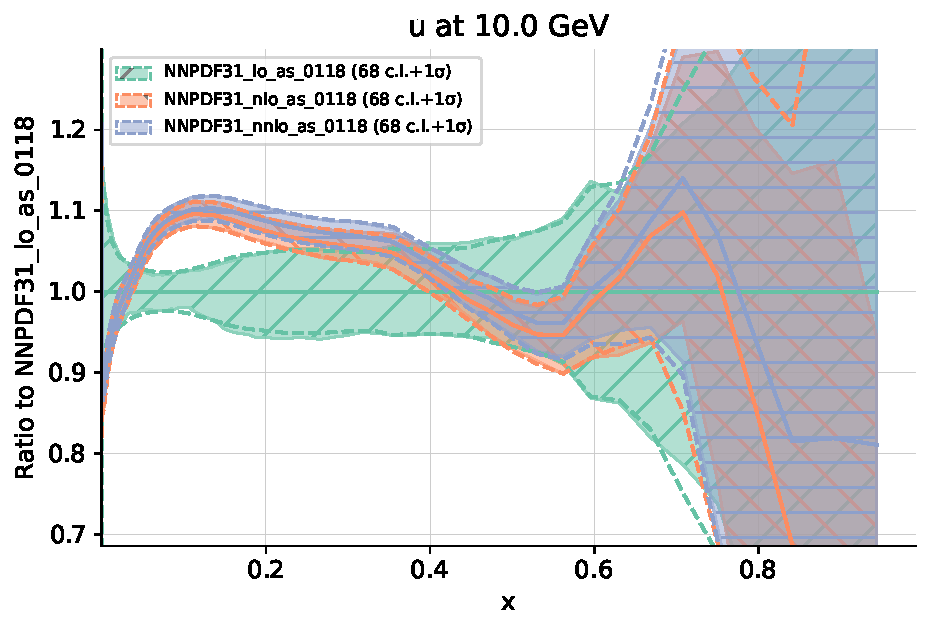
\includegraphics[width=0.49\linewidth]{mhous/plots/pdfscalespecs1_basespecs0_pdfnormalize1_plot_pdfs_u.pdf}
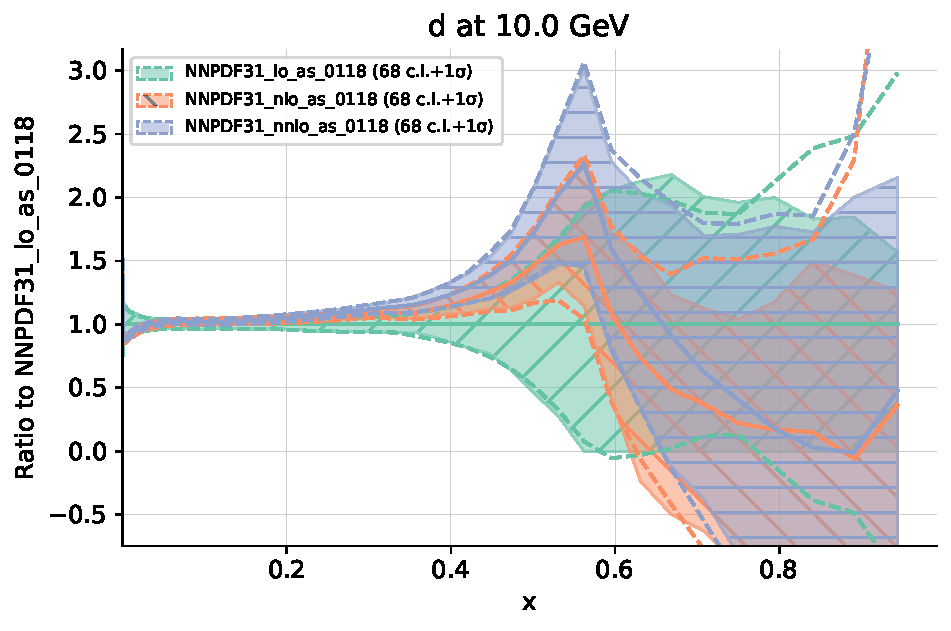
\includegraphics[width=0.49\linewidth]{mhous/plots/pdfscalespecs1_basespecs0_pdfnormalize1_plot_pdfs_d.pdf}\\
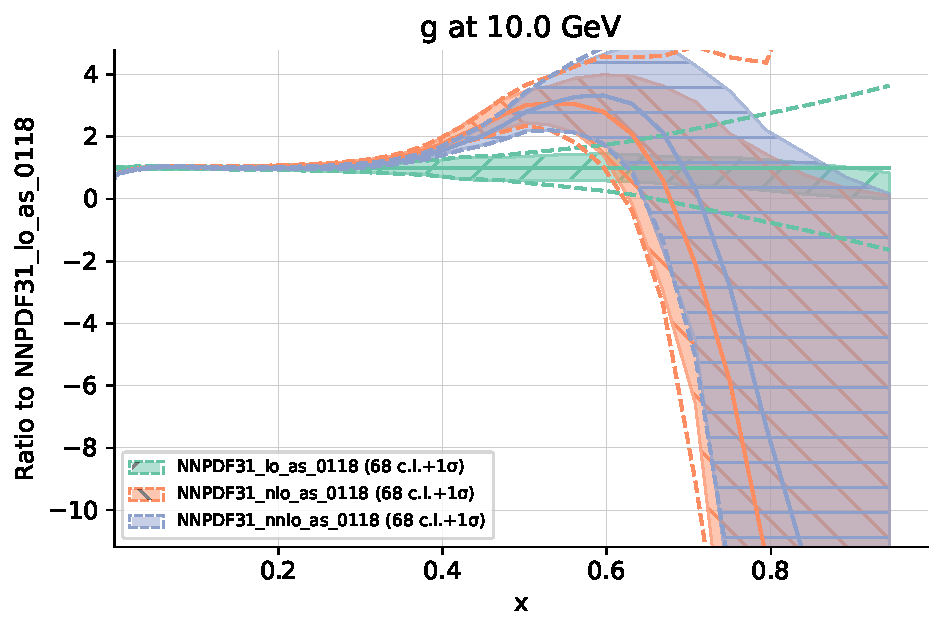
\includegraphics[width=0.49\linewidth]{mhous/plots/pdfscalespecs1_basespecs0_pdfnormalize1_plot_pdfs_g.pdf}
\caption{Comparison of NNPDF3.1 PDFs at different perturbative orders: LO (green); NLO (orange); NNLO (blue). PDFs are normalised to the LO result, and displayed at scale $Q$ = 10 GeV.}
\label{fig:pdf_order_comp}
\end{figure}

In addition to a missing source of per-point uncertainty on each data point, MHOUs can affect a PDF fit more insidiously by impacting on the desired weight of data sets relative to one another; regions of data with high MHOU are naturally to be trusted less when used to determine the PDFs, and so should carry less weight in the fitting process. If MHOUs are included, these data will be deweighted automatically because they will carry higher uncertainty, however in the absence of MHOUs they may impact on a fit to an undesirable degree.

Having established the importance of including MHOUs, in the next section we will go on to develop a formalism for estimating them, and constructing a MHOU covariance matrix.

\section{Scale variation}
\label{sec:svn}

\subsection{Renormalisation group invariance}

\subsection{Scale variation in partonic cross sections}
\subsubsection{Electroproduction}
\subsubsection{Hadroproduction}

\subsection{Scale variation in evolution of PDFs}
\subsection{Varying two scales together}
\subsubsection{Electroproduction}
\subsection{Hadroproduction}

\subsection{Scale variation for two processes}

\section{Building the theory covariance matrix}
\label{sec:prescrip}
\subsection{Symmetric prescriptions}
\subsection{Asymmetric prescriptions}
\subsection{Categorising processes}
\subsection{NLO theory covariance matrices}

\section{Validating the theory covariance matrix}
\label{sec:valid}

\section{PDFs with missing higher order uncertainties}
\label{sec:pdfs}

\section{Impact on phenomenology}
\label{sec:mhoupheno}
